\documentclass[a4paper]{article}
\usepackage[svgnames]{xcolor}
\usepackage{amsmath,amsfonts,amssymb}
\usepackage{geometry}
\usepackage{fancyhdr}
\usepackage{graphicx}
\usepackage{titlesec}
\usepackage{caption}
\usepackage{subcaption}
\usepackage{tikz}
\usepackage{tcolorbox}
\usepackage{float} % For figure positioning
\usepackage{lipsum}
\usepackage{mdframed}
\usepackage{amsmath}
\usepackage{amsmath,amsfonts,amssymb}
\usepackage{graphicx}
\usepackage{enumitem}
\usepackage{titlesec}
\usepackage{fancyhdr}
\usepackage{hyperref}
% \usepackage{floatrow}
\usepackage{listings}
\usepackage{geometry}
\usepackage{fancyhdr}
\usepackage{empheq}
\usepackage{xpatch}
\usepackage{listings}

\lstdefinestyle{Matlab}{
    language=Matlab,                      % Use MATLAB language
    basicstyle=\ttfamily\footnotesize,    % Font size and style
    keywordstyle=\color{blue},            % Color for keywords
    stringstyle=\color{red},              % Color for strings
    commentstyle=\color{green!50!black},  % Color for comments
    numbers=left,                         % Line numbers on the left
    numberstyle=\tiny\color{gray},        % Style of line numbers
    stepnumber=1,                         % Line numbers step
    numbersep=5pt,                        % Distance from line numbers
    frame=single,                         % Frame around the code
    tabsize=4,                            % Set tab size
    breaklines=true,                      % Automatic line breaking
    captionpos=b                          % Position of the caption
}


\geometry{margin=0.5in}
\pagestyle{fancy}
\fancyhf{}

% Header and Footer
% \fancyhead[L]{\includegraphics[width=1.5cm]{logo.png}} % Add your logo
\fancyhead[C]{\textbf{\color{blue!70}CS663 Assignment-3}}
% \fancyhead[R]{\color{blue!70}Saksham Rathi}
\fancyfoot[C]{\thepage}

% Custom Section Color and Format
\titleformat{\section}
{\color{purple!80!black}\normalfont\Large\bfseries}
{\thesection}{1em}{}

% Beautiful Title with TikZ
\newcommand{\cooltitle}[1]{%
  \begin{tikzpicture}
    \node[fill=blue!20,rounded corners=10pt,inner sep=10pt] (box)
    {\Huge \bfseries \color{black} #1};
  \end{tikzpicture}
}

% Stylish Solution Environment with float option enabled
% Stylish Solution Environment with breakable option
% Stylish Solution Environment with mdframed
\newenvironment{solution}[2][]{%
    \begin{mdframed}[linecolor=green!60!black, linewidth=2pt, roundcorner=10pt, backgroundcolor=green!5!white, skipabove=12pt, skipbelow=12pt]%
        \textbf{\large #2} % Heading in bold and large font
        \par\noindent\rule{\textwidth}{0.4pt} % Horizontal line after heading
        \vspace{0.5em} % Small vertical space
}{%
    \end{mdframed}%
}





\title{\cooltitle{CS663 Assignment-3}}
\author{{\bf Saksham Rathi, Kavya Gupta, Shravan Srinivasa Raghavan} \\
\small Department of Computer Science, \\
Indian Institute of Technology Bombay \\}
\date{}

\begin{document}

\maketitle
\section*{Question 1}

\begin{solution}{Solution}
    \textbf{Note:} All the Fourier Transform and Frequency Response figures are shown in logarithm absolute format.

    \subsection*{Original Image}
    \begin{figure}[H]
        \begin{subfigure}{.45\textwidth}
        \centering
          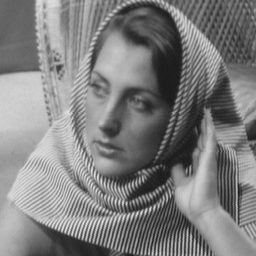
\includegraphics[width=1\linewidth]{../images/barbara256.png}
          \caption{Original Image}
        \end{subfigure}
        \begin{subfigure}{.5\textwidth}
        \centering
          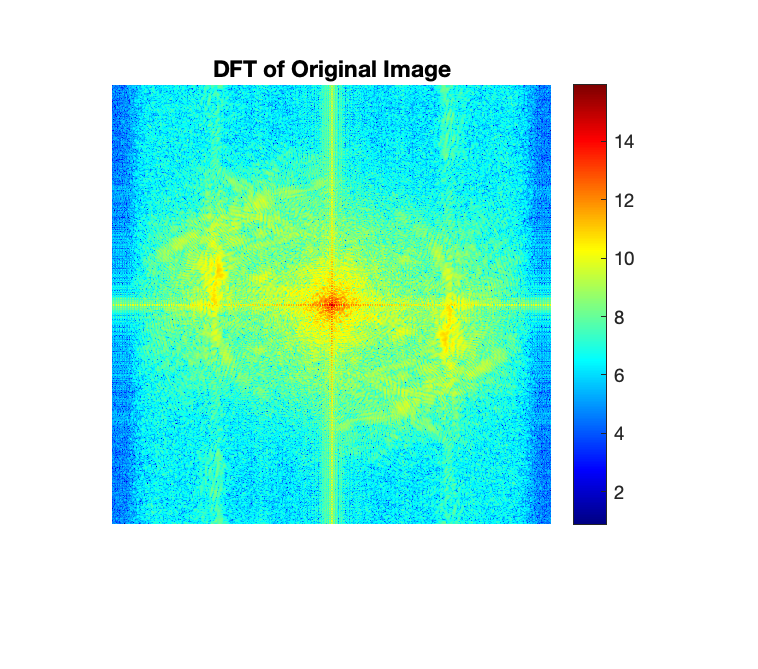
\includegraphics[width=1\linewidth]{../images/barbara_original_DFT.png}
          \caption{Fourier Transform of Original Image}
        \end{subfigure}
    \end{figure}
    
    \subsection*{Ideal Low Pass Filter}
    
    \subsubsection*{Cutoff Frequency = 40}
    \begin{figure}[H]
        \begin{subfigure}{.45\textwidth}
        \centering
          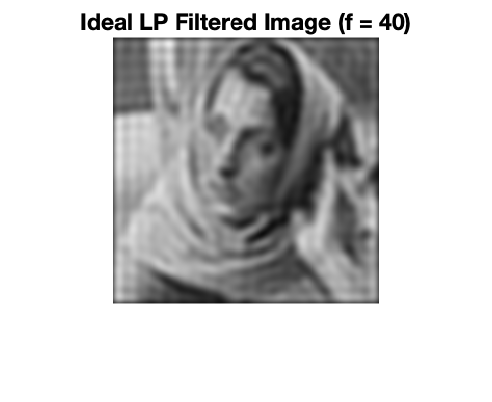
\includegraphics[width=1\linewidth]{../images/barbara_ideal_LPF_40.png}
          \caption{Filtered Image}
        \end{subfigure}
        \begin{subfigure}{.5\textwidth}
        \centering
          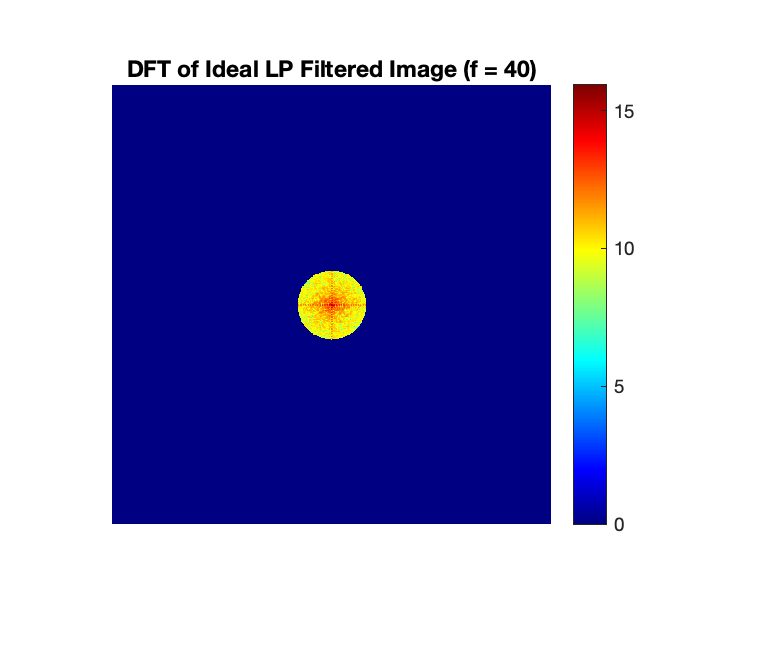
\includegraphics[width=1\linewidth]{../images/barbara_DFT_ideal_LPF_40.png}
          \caption{Fourier Transform of Filtered Image}
        \end{subfigure}
    \end{figure}
    
    \begin{figure}[H]
        \centering
        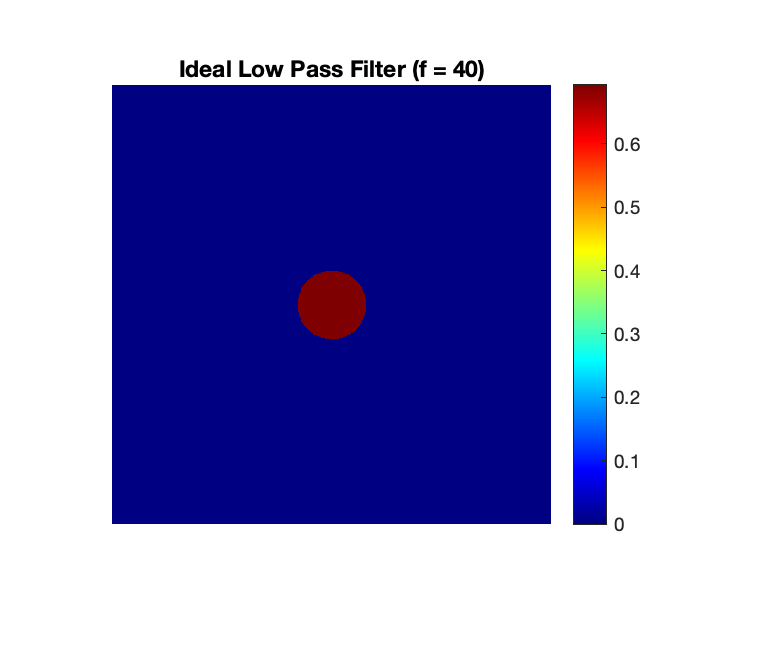
\includegraphics{../images/ideal_LPF_40.png}
        \caption{Frequency Response of Filter}
    \end{figure}
    
    \subsubsection*{Cutoff Frequency = 80}
    \begin{figure}[H]
        \begin{subfigure}{.45\textwidth}
        \centering
          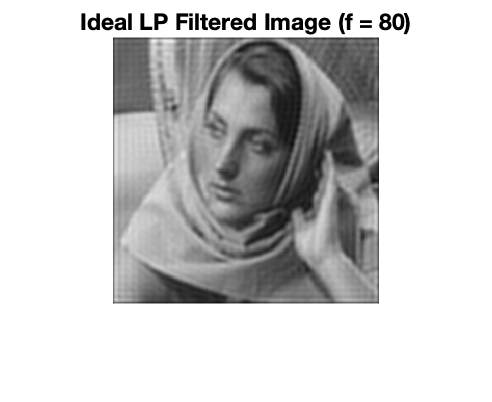
\includegraphics[width=1\linewidth]{../images/barbara_ideal_LPF_80.png}
          \caption{Filtered Image}
        \end{subfigure}
        \begin{subfigure}{.5\textwidth}
        \centering
          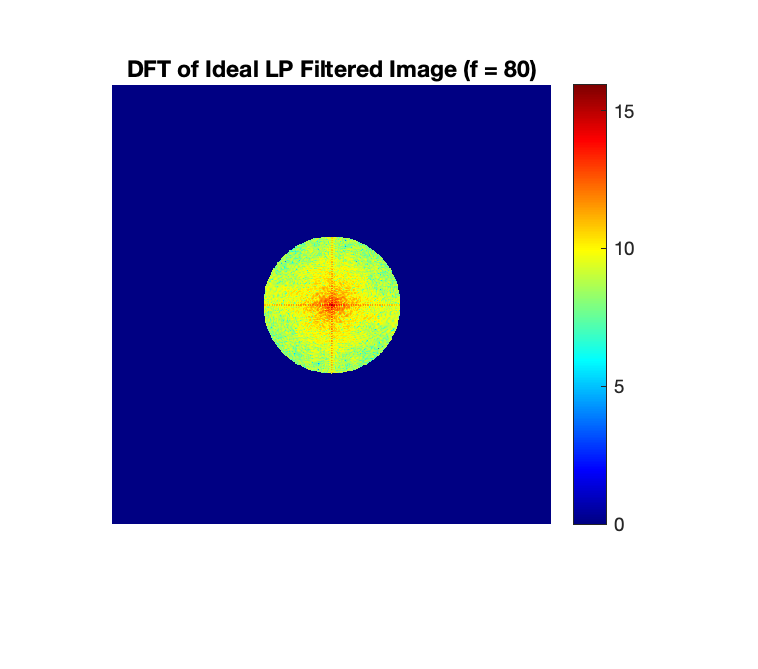
\includegraphics[width=1\linewidth]{../images/barbara_DFT_ideal_LPF_80.png}
          \caption{Fourier Transform of Filtered Image}
        \end{subfigure}
    \end{figure}
    
    \begin{figure}[H]
        \centering
        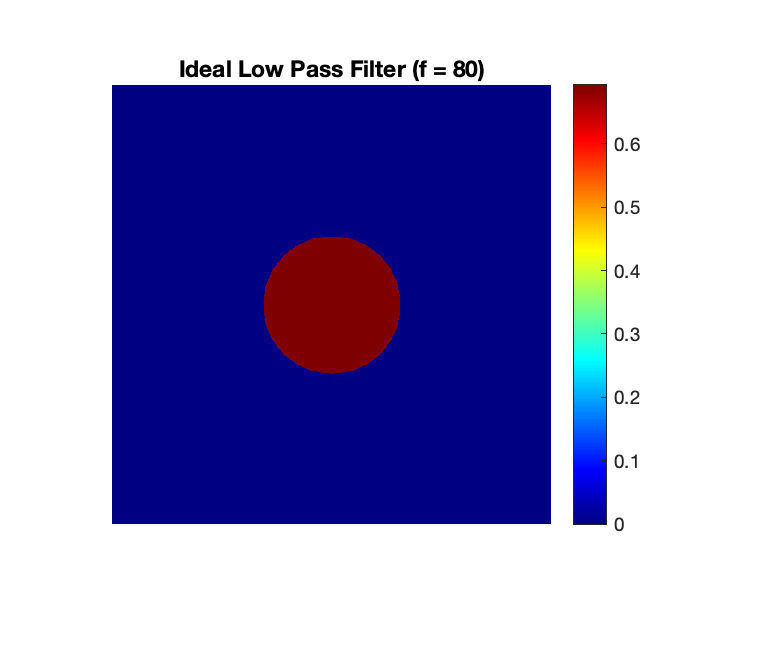
\includegraphics{../images/ideal_LPF_80.png}
        \caption{Frequency Response of Filter}
    \end{figure}
    
    \subsection*{Gaussian Low Pass Filter}
    
    \subsubsection*{Sigma = 40}
    \begin{figure}[H]
        \begin{subfigure}{.45\textwidth}
        \centering
          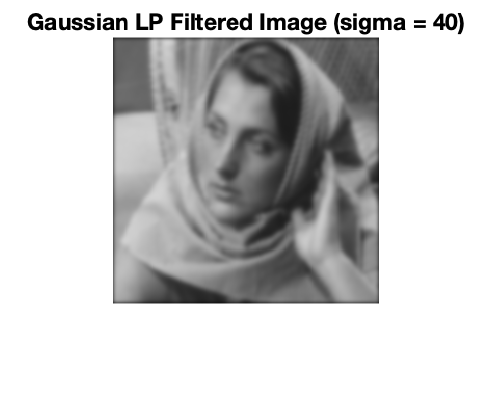
\includegraphics[width=1\linewidth]{../images/barbara_gaussian_LPF_40.png}
          \caption{Filtered Image}
        \end{subfigure}
        \begin{subfigure}{.5\textwidth}
        \centering
          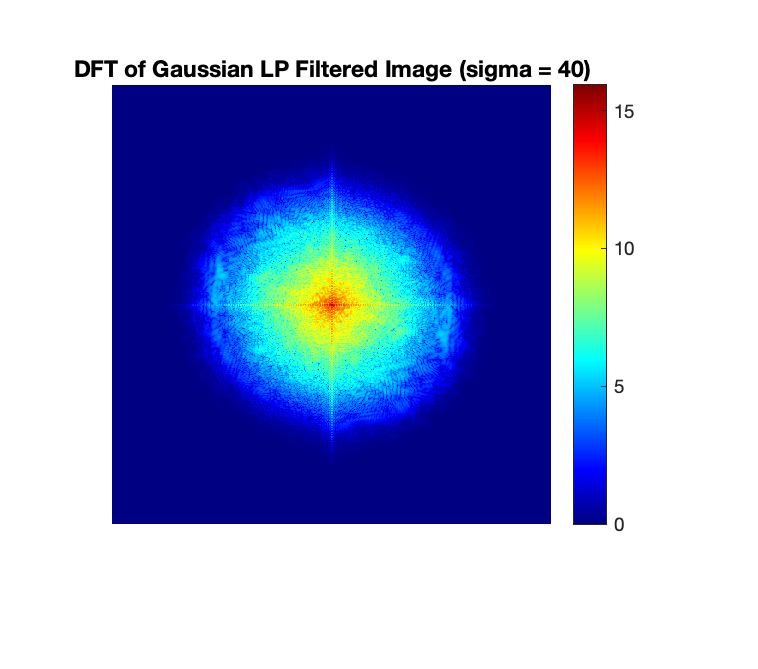
\includegraphics[width=1\linewidth]{../images/barbara_DFT_gaussian_LPF_40.png}
          \caption{Fourier Transform of Filtered Image}
        \end{subfigure}
    \end{figure}
    
    \begin{figure}[H]
        \centering
        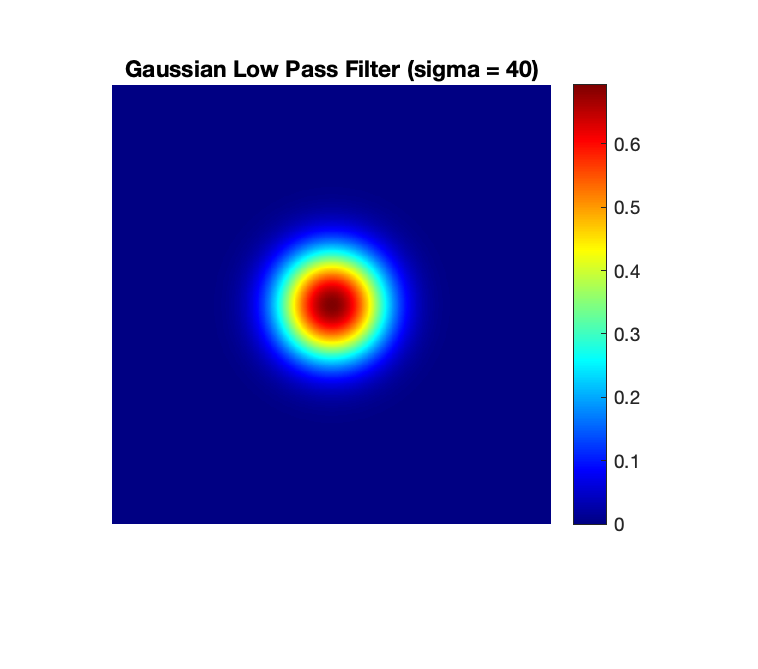
\includegraphics{../images/gaussian_LPF_40.png}
        \caption{Frequency Response of Filter}
    \end{figure}
    
    \subsubsection*{Sigma = 80}
    \begin{figure}[H]
        \begin{subfigure}{.45\textwidth}
        \centering
          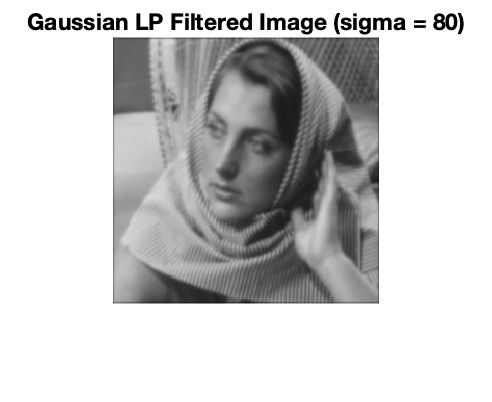
\includegraphics[width=1\linewidth]{../images/barbara_gaussian_LPF_80.png}
          \caption{Filtered Image}
        \end{subfigure}
        \begin{subfigure}{.5\textwidth}
        \centering
          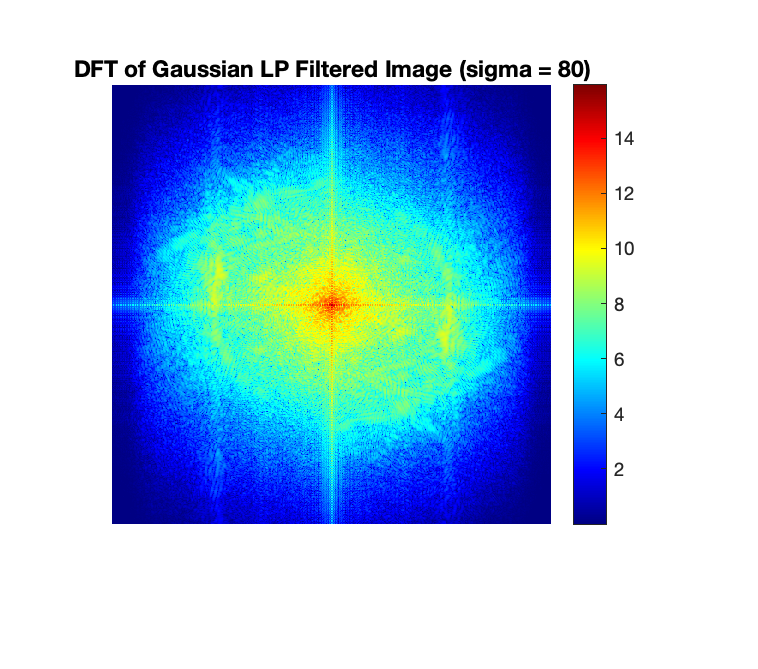
\includegraphics[width=1\linewidth]{../images/barbara_DFT_gaussian_LPF_80.png}
          \caption{Fourier Transform of Filtered Image}
        \end{subfigure}
    \end{figure}
    
    \begin{figure}[H]
        \centering
        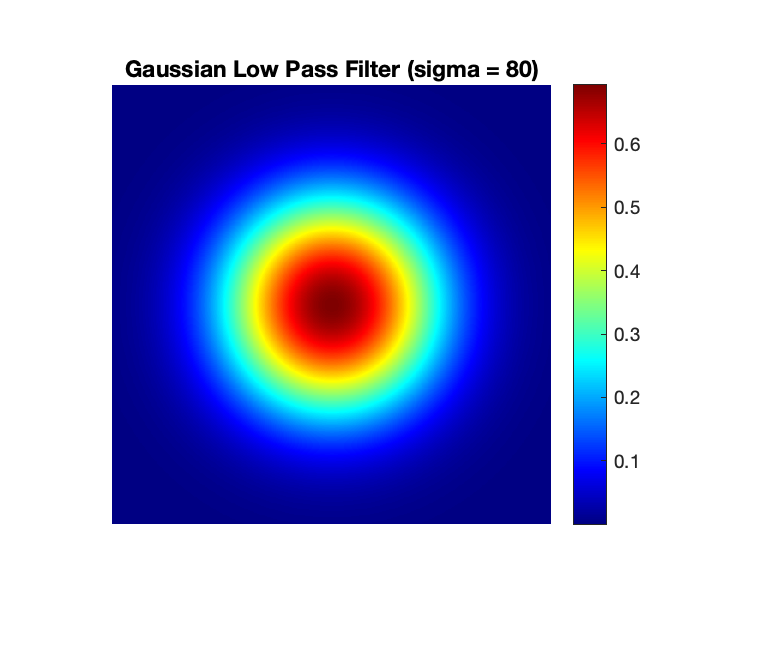
\includegraphics{../images/gaussian_LPF_80.png}
        \caption{Frequency Response of Filter}
    \end{figure}
    
    \subsection*{Observations}
    
    \begin{itemize}
        \item From the obtained results we can easily see that as the cut-off frequency (for ideal low pass
        filter) / sigma (for Gaussian low pass filter) is increased, the higher frequency components
        which correspond to finer details in the image start becoming clearly visible.
        \item Also we can see that for ideal low pass filter there is a presence of \textbf{ringing artifacts} that appear
        as spurious signals near sharp transitions in the images. These ringing artifacts are quite
        undesirable and are a result of the complete elimination of high frequencies higher than the
        cut-off frequency by the ideal low pass filter.
        \item When a Gaussian low pass filter is used these ringing artifacts are absent.\ This is because the
        Gaussian low pass filter does not completely eliminate the higher frequencies and rather weakens
        them.
    \end{itemize}
\end{solution}


\end{document}
